\documentclass{article}% [Determines font size] { }Determines type of document (article/beamer/book/etc.)

\usepackage{graphicx}% Required package to compile figures.

\begin{document}% Required to produce a compiled LaTeX document. 


Figure 0: Simple Figure format. \\
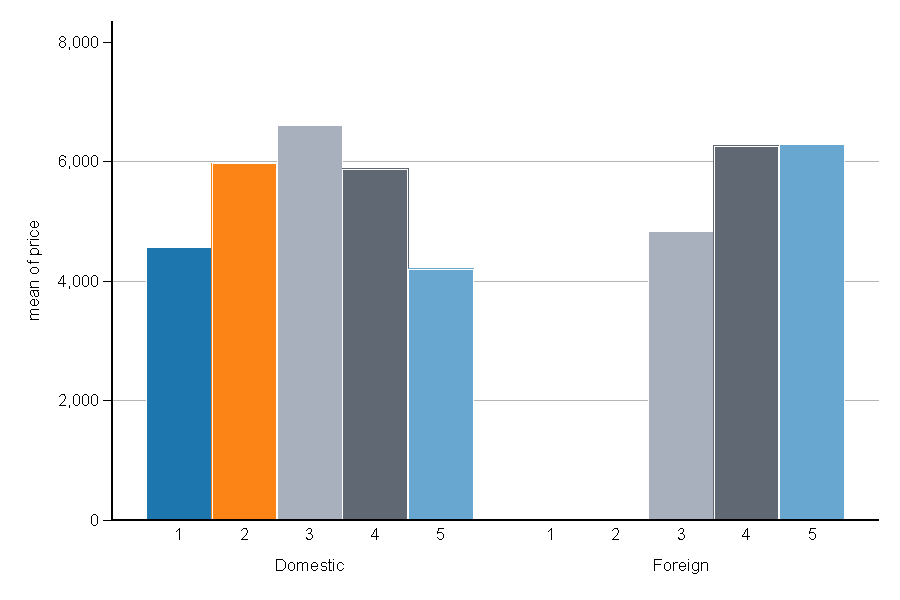
\includegraphics{figure1.pdf}

This is a very simple code that will just drop the figure in the current environment in its original form.
\newpage


\begin{figure}[ht]% This creates a separate environment for the figure, independent of the rest of the document. [ ] are placing options of where in the page/environment should the figure be displayed, and when to overwrite other established rules. 
        \caption{Complete figure format}% Creates a title for the figure, with an automatically generating ordered number placement of the figure. To place the title below the figure, then place the \caption command after \includegraphics.
        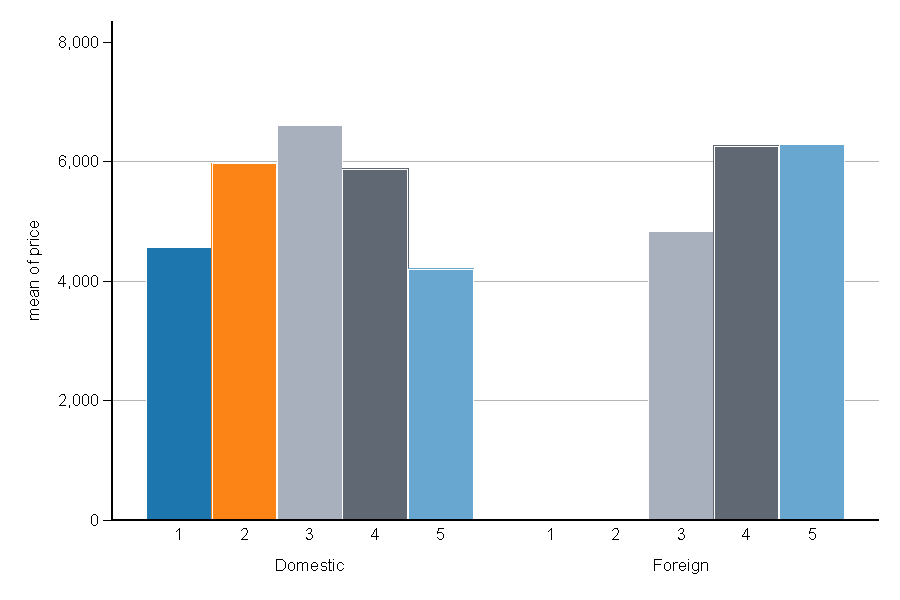
\includegraphics[height=5.2287in, width=6.4377in]{figure1.pdf}% [ ] used to customize the size of the figure displayed in document. 
        \label{fig:absolute}%Use a ":" to create a category of labels on the left side, and the right side is the label of this specific figure.
\end{figure}

This is a standard way of printing a figure, with a separate figure environment, which allows the user to have more control over where it is placed within the page and causing minimal disruption to other rules governing the document. 
\newpage


\begin{figure}[ht]
        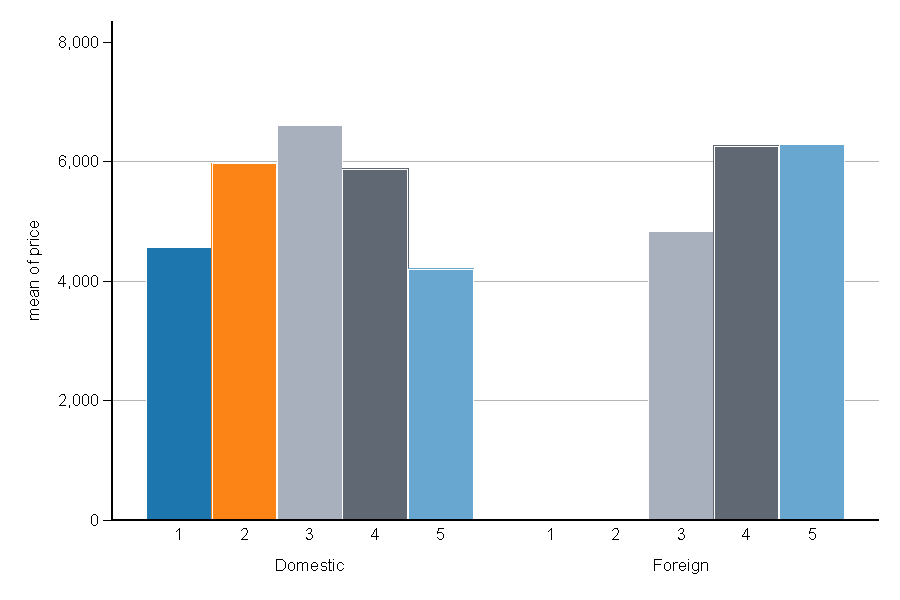
\includegraphics[width=.5\textwidth]{figure1.pdf}% Alternative method of determining size of figure as a relational size instead of absolute size.
        \caption{50\% Textwidth figure}
        \label{fig:relative}
\end{figure}

Sizing of figure can be done based on absolute size, or by relative size. Also Title is below figure here.

\end{document}